\documentclass[12pt,a4paper]{ctexrep}
\usepackage[top=2cm,bottom=2cm,left=2.5cm,right=2.5cm]{geometry}
\usepackage{graphicx}
\usepackage{booktabs}
\usepackage{array}
\usepackage{amsmath}
\usepackage{amssymb}
\usepackage{multirow}
\usepackage{float}
\usepackage{caption}
\usepackage{hyperref}
\usepackage{setspace}
\usepackage{fancyhdr}
\setlength{\headheight}{14pt}
\usepackage{tabu}
\usepackage{longtable}
\usepackage{subcaption}

\graphicspath{{../figures/}}
\onehalfspacing

\pagestyle{fancy}
\fancyhf{}
\fancyhead[C]{\small 第十届全国密码技术竞赛——作品设计报告}
\fancyfoot[C]{\thepage}

\ctexset{
  chapter/name = {,.},
  chapter/number = \arabic{chapter}
}
\hypersetup{colorlinks=true,linkcolor=black,citecolor=black}

\begin{document}

% ============= 封面 =============
\thispagestyle{empty}
\begin{center}
  \vspace*{1cm}
  {\LARGE\bfseries 2025年第十届全国密码技术竞赛\\[0.3em] 作品设计报告}
  \vspace{2cm}

  \begin{tabu}{p{3cm}p{10cm}}
    \toprule
    \multicolumn{2}{c}{\Large\bfseries 基本信息表} \\
    \midrule
    作品题目： & \bfseries 混沌置乱的循环阶分析 \\
    \midrule
    作品类别： &
    $\blacksquare$ 软件设计 \quad $\square$ 硬件制作 \quad $\square$ 工程实践 \quad
    $\square$ 密码技术应用 \quad $\square$ 其它 \\
    \midrule
    作品内容摘要： &
    置乱操作是许多密码算法和图像加密方案的核心步骤。传统置乱表生成依赖伪随机数发生器，
    本文系统研究基于混沌映射生成置乱表的方法及其循环结构特性。选取 Logistic、Tent、
    Chebyshev、Sine 和 Henon 五种不同类型混沌映射，通过迭代预热、排序索引法生成置乱表，
    对置乱表进行循环分解并计算置换阶（LCM）。设计六项实验（E1--E6）全面评测其密码安全性，
     包括平均阶规模、循环分布、种子初值敏感性、有限精度退化、排序偏差及参数敏感性。
     实验结果表明：混沌排序置乱在循环结构上接近均匀随机置换，
    但低精度实现（float32）会显著降低置换阶。值得注意的是，排序索引法（argsort）本身会部分抹除混沌序列的结构特征，最终置换的统计特性由 argsort 主导。
    \\
    \midrule
    关键词（五个）： &
    混沌映射；置乱；循环分解；置换阶；密码安全 \\
    \bottomrule
  \end{tabu}
\end{center}

\vfill
\begin{center}
  年 \quad 月 \quad 日
\end{center}

\vfill
\begin{center}
  中国密码学会
\end{center}

\newpage

% ============= 目录 =============
\tableofcontents
\newpage

% ============= 第1章 作品功能与性能说明 =============
\chapter{作品功能与性能说明}

本作品开发了一套基于混沌映射的置乱表生成与循环分析软件，
主要功能涵盖以下方面：

\begin{enumerate}
  \item \textbf{多类型混沌映射库}：集成五种不同类型的混沌映射——
  Logistic（二次多项式型）、Tent（分段线性型）、Chebyshev（正交多项式型）、
  Sine（超越函数型）和 Henon（二维映射型），覆盖混沌理论的主要分类。
  每种映射均支持参数调节和种子设定。

  \item \textbf{置乱表生成}：采用排序索引法（argsort）生成置换表。
  实现 M=1000 轮预热消除暂态，支持任意规模 N 的置乱表生成。
  生成的置换表通过双射校验，确保数学正确性。

  \item \textbf{循环结构分析}：对生成的置乱表进行完全循环分解，
  统计各循环长度出现频次、计算置换阶（所有循环长度的最小公倍数）。
  支持超大阶的对数化处理（$\ln(\text{order})$），避免大整数溢出。

  \item \textbf{密码安全性评估}：设计六项系统性实验（E1--E6），
  从平均阶规模、循环分布特征、种子雪崩效应、有限精度退化效应、
  排序法偏差分析和参数敏感性等多个维度，全面评估混沌置乱的密码安全性。
\end{enumerate}

本软件支持 N=64 至 4096 的置乱规模，每组实验默认 100 组独立种子，
确保统计结果的可靠性。所有实验数据以 CSV 格式输出，图形以 PNG 格式保存，
方便进一步分析和报告撰写。

% ============= 第2章 设计与实现方案 =============
\chapter{设计与实现方案}

\section{实现原理}

\subsection{混沌映射}

本作品选取五种不同类型的混沌映射，覆盖混沌理论的主要分类体系。
各映射函数接口统一为 $\text{func}(\text{seed}, n) \rightarrow \mathbb{R}^n$。

\begin{table}[H]
  \centering
  \caption{符号说明}
  \begin{tabular}{cl}
    \toprule
    符号 & 含义 \\
    \midrule
    $N$ & 置乱规模（置换长度） \\
    $M = 1000$ & 预热轮数，消除暂态 \\
    $\pi$ & 置换表，$\pi \in S_N$ \\
    $\mathrm{ord}(\pi)$ & 置换阶，$\mathrm{lcm}$ 所有循环长度 \\
    $\mathbb{E}[\ln O]$ & 对数阶的样本均值，$\frac{1}{K}\sum\ln(\mathrm{ord}(\pi_k))$ \\
    $\mu, r, a, b$ & 各混沌映射的控制参数 \\
    \bottomrule
  \end{tabular}
\end{table}

\subsubsection*{Logistic 映射}
\begin{equation}\label{eq:logistic}
  x_{n+1} = \mu x_n (1 - x_n),\quad \mu = 3.99,\; x \in (0,1)
\end{equation}
Logistic 映射是经典的二次多项式混沌系统。当 $\mu \in (3.57, 4]$ 时系统处于混沌状态，
本作品取 $\mu = 3.99$ 以保证充分的混沌行为。

\subsubsection*{Tent 映射}
\begin{equation}\label{eq:tent}
  x_{n+1} = r \cdot \begin{cases}
    x_n, & x_n < 0.5 \\
    1 - x_n, & x_n \ge 0.5
  \end{cases},\quad r = 1.99
\end{equation}
Tent 映射是分段线性混沌映射，结构简单，但具有与 Logistic 映射不同的混沌动力学特征。

\subsubsection*{Chebyshev 映射}
\begin{equation}\label{eq:chebyshev}
  x_{n+1} = T_3(x_n) = 4x_n^3 - 3x_n,\quad x \in (-1, 1)
\end{equation}
采用 $k=3$ 阶 Chebyshev 多项式的等价代数形式（$T_3$ 为最低阶非平凡 Chebyshev 映射），
避免 $\cos(\arccos x)$ 的浮点域问题。

\subsubsection*{Sine 映射}
\begin{equation}\label{eq:sine}
  x_{n+1} = r \sin(\pi x_n),\quad r = 0.99,\; x \in (0,1)
\end{equation}
Sine 映射属于超越函数型混沌映射。参数 $r=0.99$ 确保系统处于混沌状态。

\subsubsection*{Henon 映射}
\begin{align}
  x_{n+1} &= 1 - a x_n^2 + y_n,\quad a = 1.4 \\
  y_{n+1} &= b x_n,\quad b = 0.3
\end{align}
Henon 映射是典型的二维离散混沌系统。本作品仅取 $x_n$ 分量参与置乱索引生成，
$y_n$ 分量仅用于迭代递推。需注意 Henon attractor 的 $x$ 分量分布不均匀
（非 $(0,1)$ 上均匀分布），这一假设可能对循环统计产生影响。

\subsection{置乱表生成}

置乱表生成采用排序索引法，流程如下：

\begin{enumerate}
  \item 选定混沌映射和种子 $x_0$，迭代 $M=1000$ 轮得到 $x_M$，消除暂态。
  \item 继续迭代 $N$ 轮，得到混沌序列 $\{x_{M+1}, x_{M+2}, \ldots, x_{M+N}\}$。
  \item 对该序列执行 $\text{argsort}$ 操作，得到置换表 $\pi$：
  \begin{equation}
    \pi = \text{np.argsort}([x_{M+1}, \ldots, x_{M+N}])
  \end{equation}
  \item 验证置换表的双射性：$\text{set}(\pi) = \{0, 1, \ldots, N-1\}$。
\end{enumerate}

关于 $\text{argsort}$ 的方向：$\text{argsort}$ 返回的 $\pi^{-1}$
与题目定义的正向置换 $\pi$ 具有完全相同的循环长度集合（仅遍历方向相反），
因此循环分析结果等价。

\subsection{循环分解}

对置换表 $\pi$ 进行完全循环分解，算法如下：

\begin{enumerate}
  \item 初始化长度为 $N$ 的 $\text{visited}$ 数组为 $\text{False}$。
  \item 遍历 $i$ 从 $0$ 到 $N-1$：
    \begin{itemize}
      \item 若 $\text{visited}[i]$ 为 $\text{True}$，跳过。
      \item 否则从 $i$ 出发追踪循环：$j = \pi[j]$ 直至回到 $i$，记录长度 $L$。
      \item 统计 $\{L: \text{count}\}$。
    \end{itemize}
\end{enumerate}

\subsection{置换的阶}

置换的阶定义为所有循环长度的最小公倍数：
\begin{equation}
  \text{order} = \text{lcm}\{L_1, L_2, \ldots, L_k\}
\end{equation}

阶的数值可能极大（超过 $2^{4096}$），因此本作品统一采用对数平均：
\begin{equation}
  \overline{\ln O} = \frac{1}{K}\sum_{k=1}^{K} \ln(\text{order}_k)
\end{equation}

\subsection{理论参考曲线}

Landau 定理给出对称群 $S_N$ 中置换阶的上界（最大可能阶）：
\begin{equation}\label{eq:landau}
  \ln g(N) \sim \sqrt{\frac{N \ln N}{2}}, \quad N \to \infty
\end{equation}
其中 $g(N) = \max_{\pi \in S_N} \mathrm{ord}(\pi)$。本报告将其作为循环阶的上界参考线。

Fisher-Yates 算法生成的均匀随机置换阶的实验均值则作为随机置换期望水平的经验基线。

Golomb--Dickman 常数给出随机置换中最大循环长度的期望值：
\begin{equation}
  \mathbb{E}[L_{\max}] \approx 0.6243 \cdot N
\end{equation}

\section{运行结果}

本作品生成七张核心结果图，全面展示实验发现。

\begin{figure}[H]
  \centering
  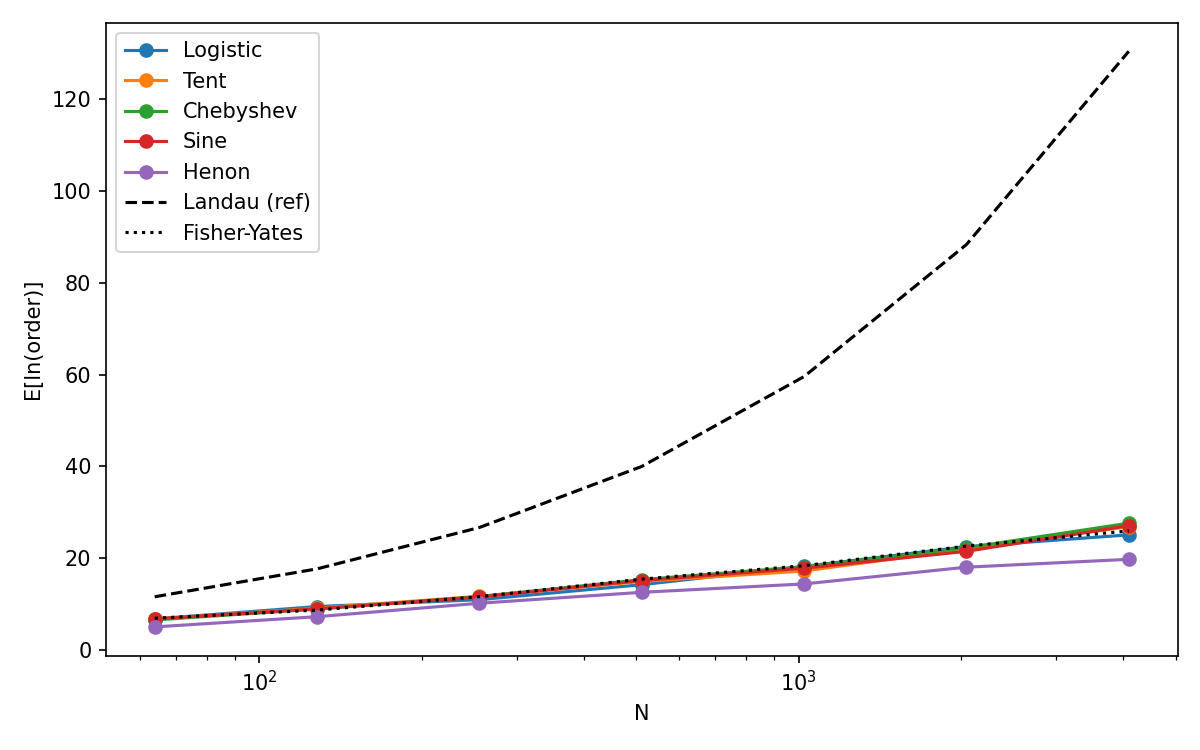
\includegraphics[width=0.9\textwidth]{fig1_avg_ln_order.png}
  \caption{五种混沌排序置乱与 Fisher-Yates 均匀随机置换的 $\mathbb{E}[\ln(\text{order})]$
  随规模 $N$ 的变化曲线，附 Landau 上界参考线和 Fisher-Yates 基线。
  各曲线与 Fisher-Yates 基线趋势一致。}
\end{figure}

\begin{figure}[H]
  \centering
  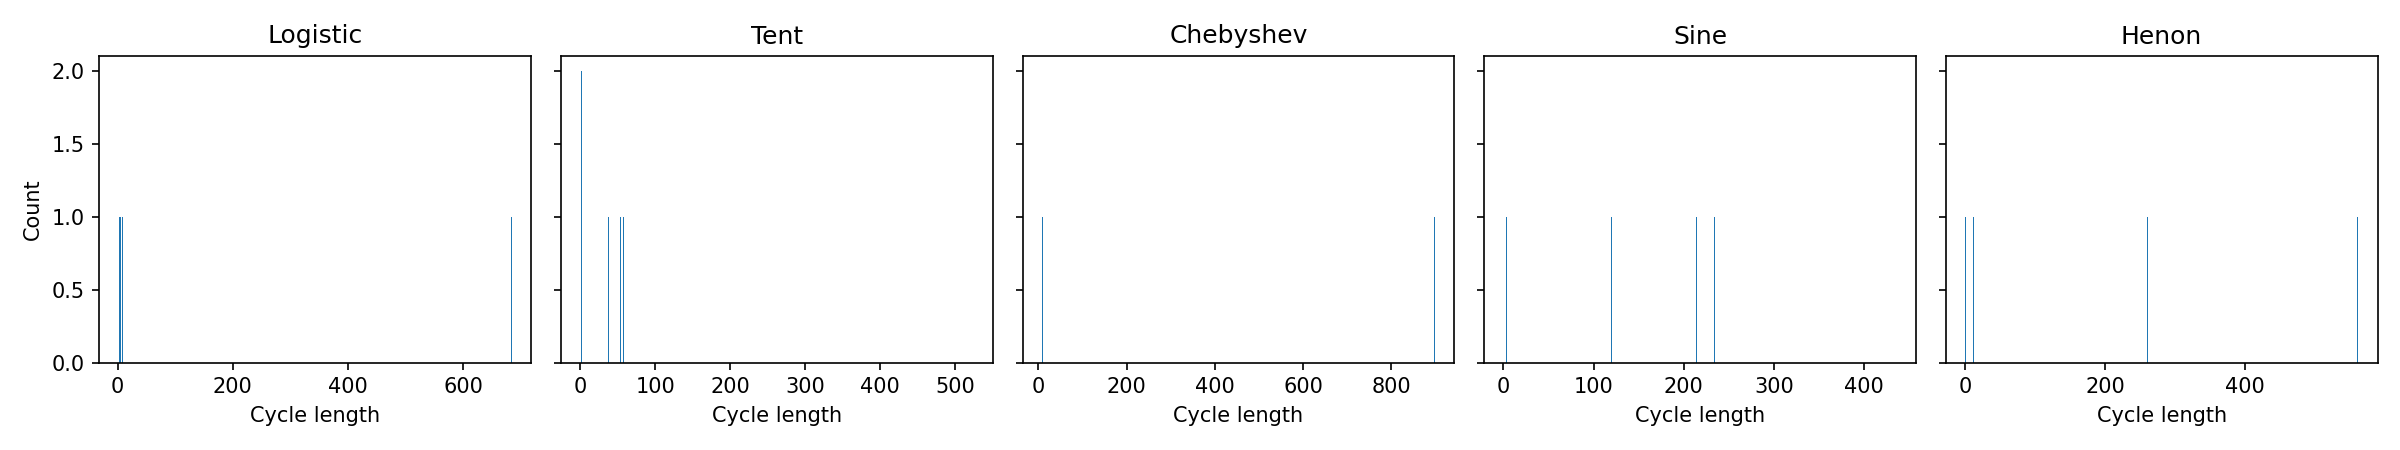
\includegraphics[width=\textwidth]{fig2_cycle_distribution.png}
  \caption{$N=1024$ 时五种映射的循环长度分布直方图。各映射的循环结构形态相似，
  以长循环为主、短循环为辅，符合均匀随机置换的循环特征。}
\end{figure}

\begin{figure}[H]
  \centering
  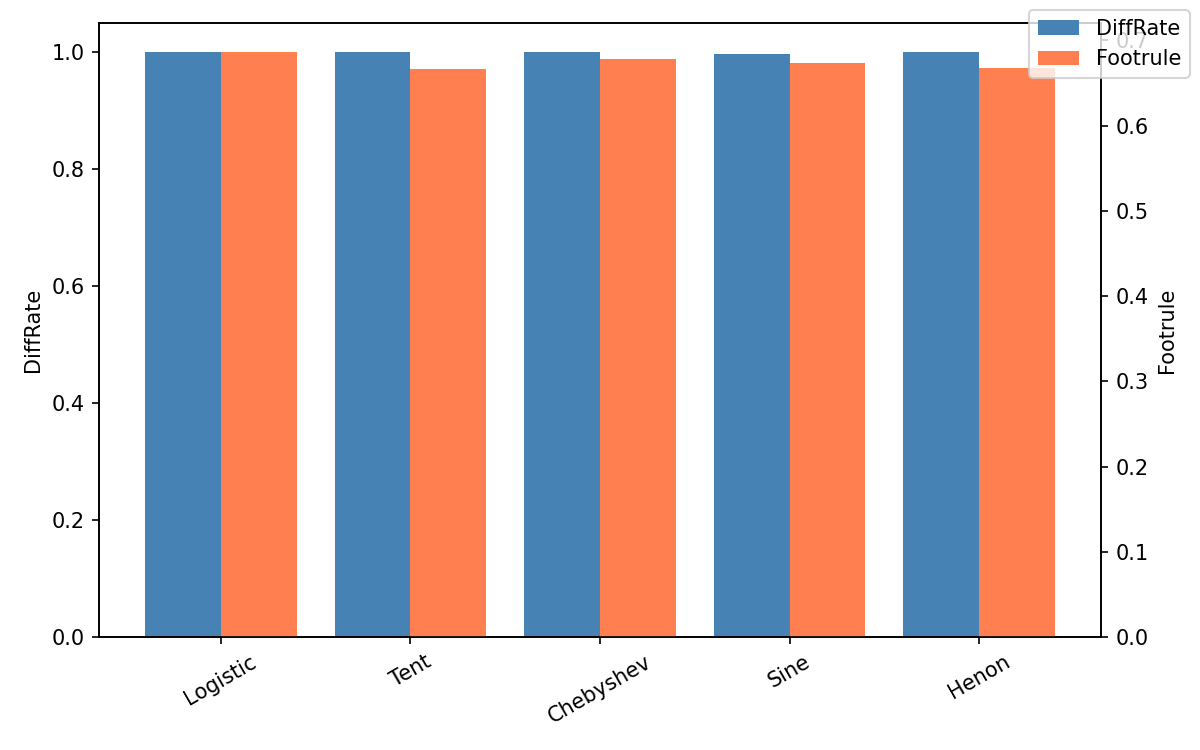
\includegraphics[width=0.8\textwidth]{fig3_seed_avalanche.png}
   \caption{种子初值敏感性实验结果。所有映射的置换差异率（DiffRate）均接近 1，
  Spearman Footrule 在 0.66--0.69 之间，表明混沌置换具有极强的初值敏感性。}
\end{figure}

\begin{figure}[H]
  \centering
  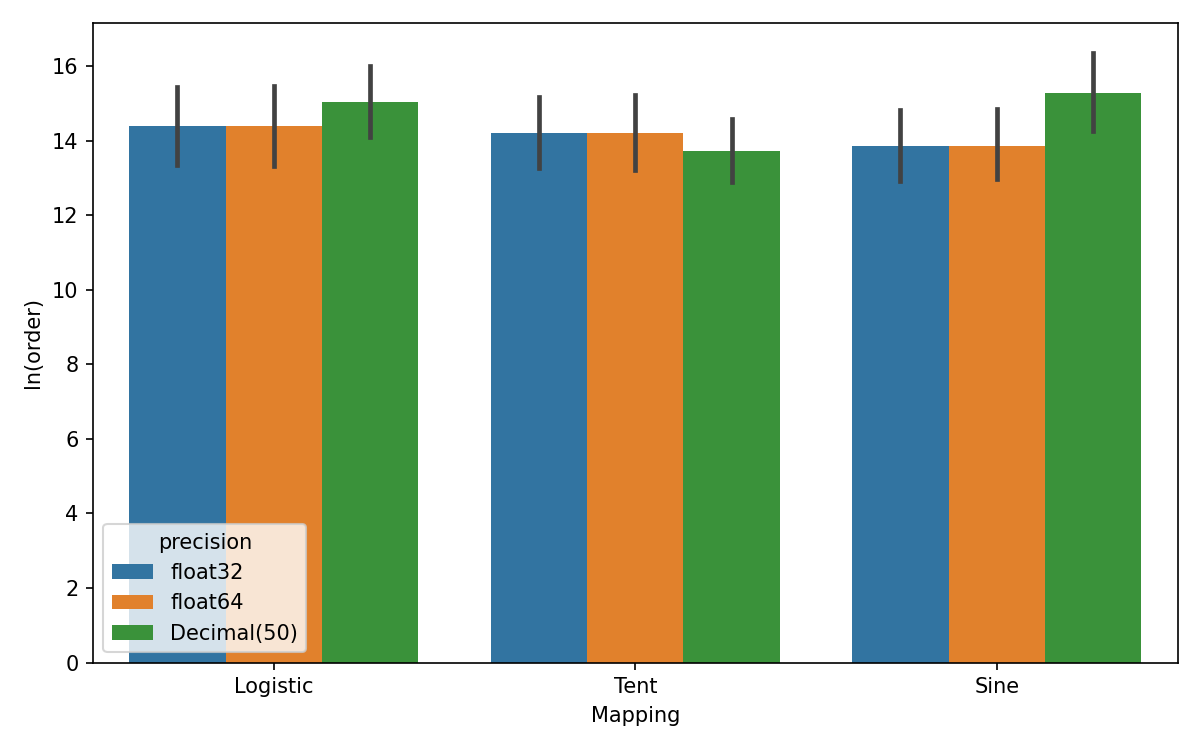
\includegraphics[width=0.8\textwidth]{fig4_precision_degradation.png}
  \caption{不同浮点精度下 $\ln(\text{order})$ 对比。float32 精度的置换阶显著低于
  float64 和 Decimal(50)，说明低精度实现会严重削弱混沌置乱的循环安全性。}
\end{figure}

\begin{figure}[H]
  \centering
  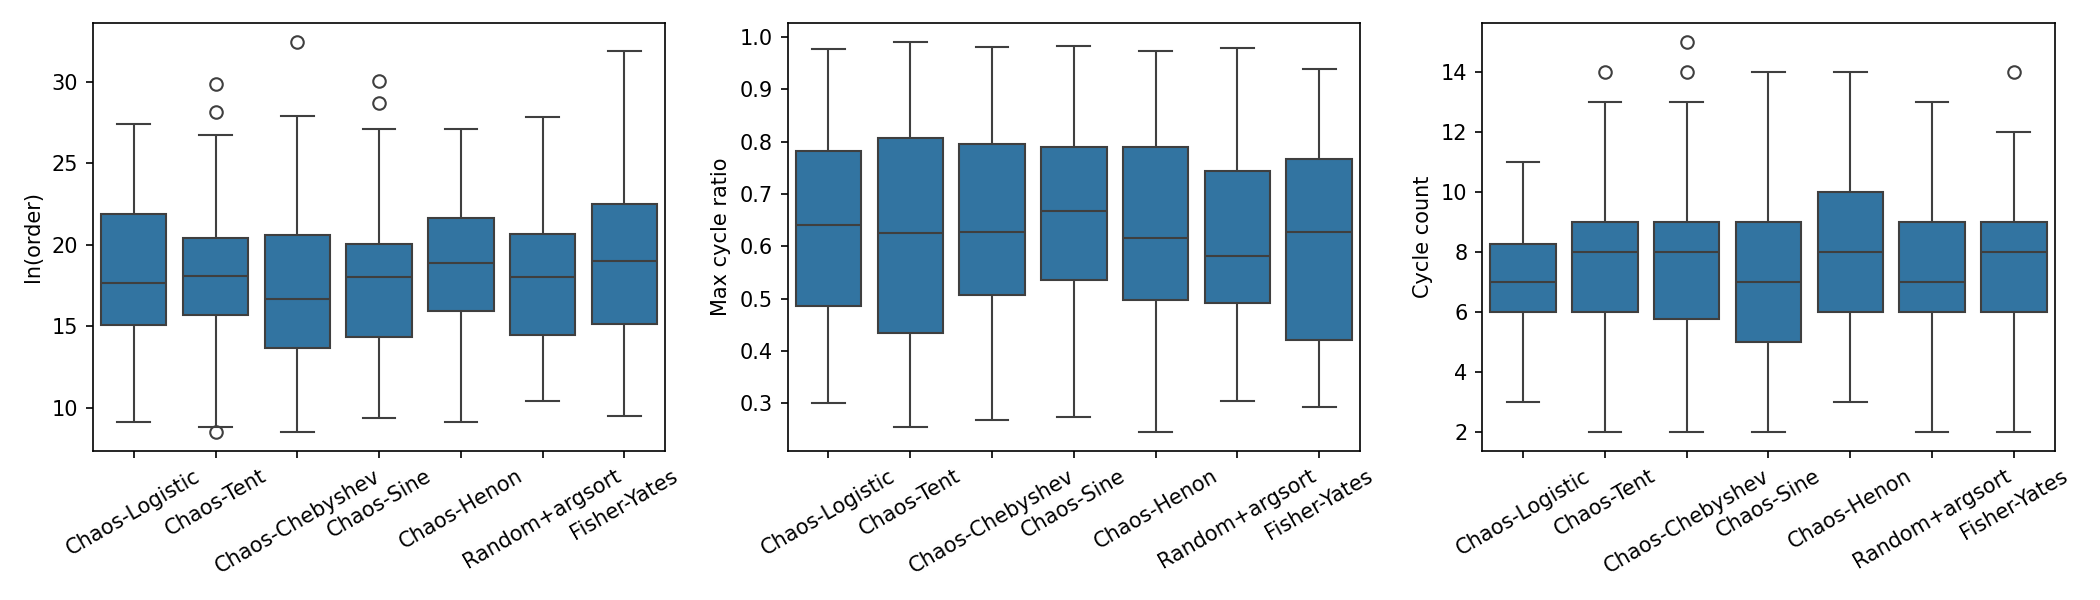
\includegraphics[width=\textwidth]{fig5_sorting_bias.png}
  \caption{排序法偏差分析箱线图。Chaos+argsort 与 Random+argsort、
  Fisher-Yates 三组的阶、最大循环比和循环数分布相近，
  说明 argsort 操作抹除了混沌序列的大部分结构特征。}
\end{figure}

\begin{figure}[H]
  \centering
  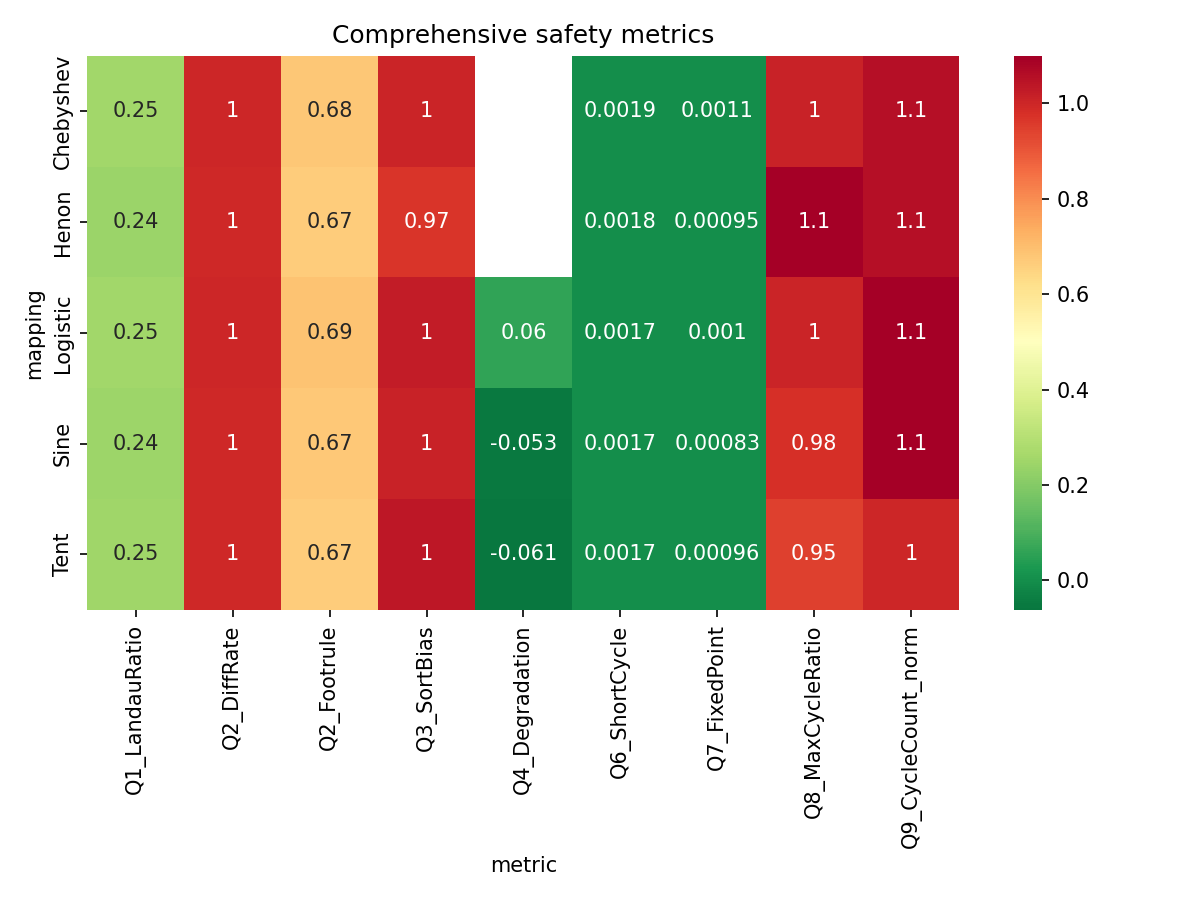
\includegraphics[width=0.7\textwidth]{fig6_summary_metrics.png}
   \caption{安全性综合评估热力图。从 Landau 比率、初值敏感性、排序偏差、
  精度退化等多个指标综合评估五种映射的安全性水平。}
\end{figure}

\begin{figure}[H]
  \centering
  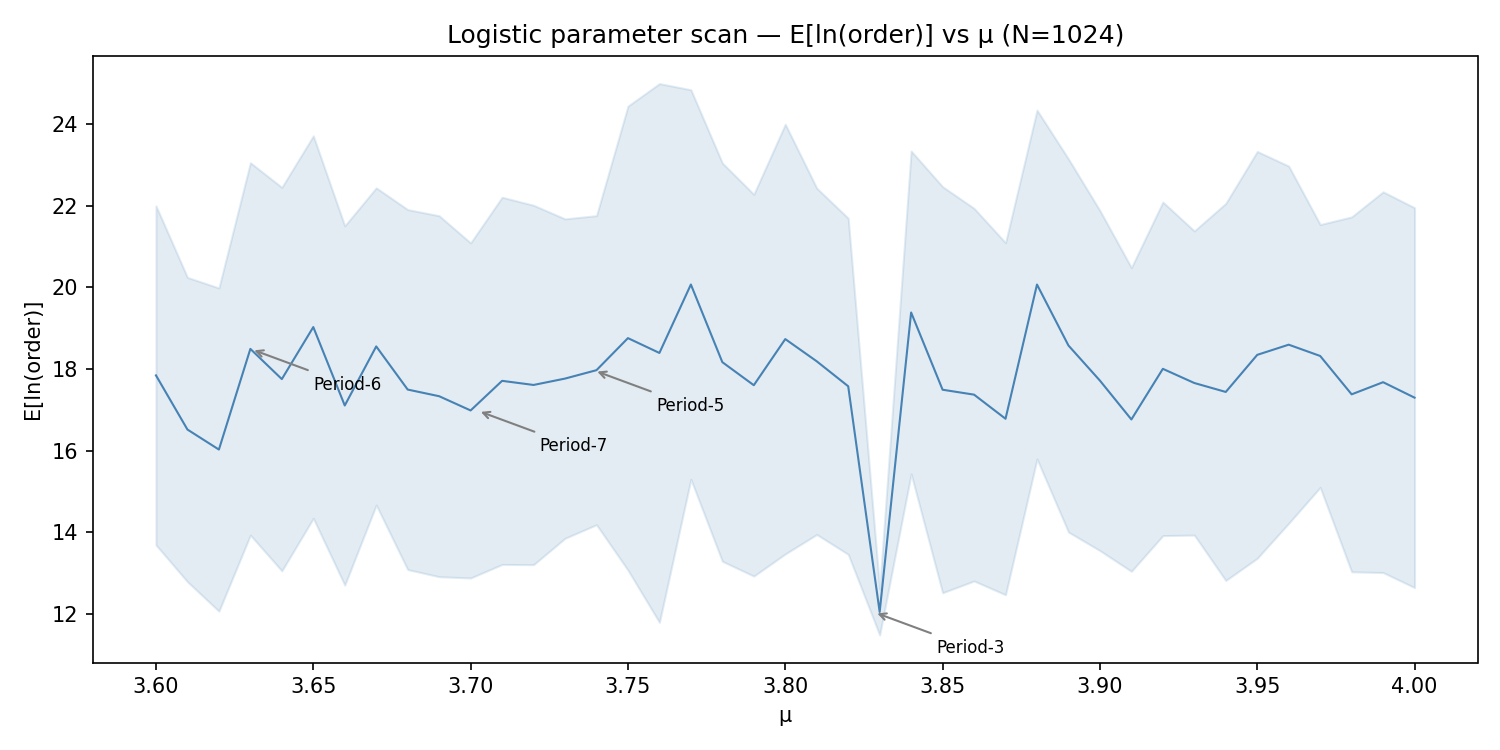
\includegraphics[width=0.8\textwidth]{fig_param_scan_logistic.png}
  \caption{Logistic 映射参数扫描结果（$N=1024$）。在 $\mu \approx 3.83$ 处
  $\mathbb{E}[\ln(\text{order})]$ 显著降低，对应周期-3 窗口。}
\end{figure}

\section{技术指标}

\begin{table}[H]
  \centering
  \caption{实验参数配置}
  \begin{tabular}{lc}
    \toprule
    参数 & 取值 \\
    \midrule
    置乱规模 $N$ & 64, 128, 256, 512, 1024, 2048, 4096 \\
    每组种子数 & 100（精度实验 30） \\
    预热轮数 $M$ & 1000 \\
    重试上限 & $\text{种子数} \times 5$ \\
    \bottomrule
  \end{tabular}
\end{table}

\begin{table}[H]
  \centering
  \caption{实验内容清单}
  \begin{tabular}{cll}
    \toprule
    编号 & 实验名称 & 目的 \\
    \midrule
    E1 & 平均阶-N 曲线 & 横向对比各映射循环特性 \\
    E2 & Landau 定理对照 & 判断是否接近随机置换水平 \\
    E3 & 种子初值敏感性 & 评测初值敏感性 \\
    E4 & 参数扫描 & 检测周期窗口（Logistic） \\
    E5 & 循环长度分布 & 展示循环结构细节 \\
    E6 & 有限精度退化 & 对比 float32/float64/Decimal \\
    E7 & 排序法偏差 & 三组对照分析 \\
    \bottomrule
  \end{tabular}
\end{table}

% ============= 第3章 系统测试与结果 =============
\chapter{系统测试与结果}

\section{测试方案}

测试平台配置：Windows 11 操作系统，Python 3.12 运行环境，
核心依赖库包括 NumPy、Pandas、Matplotlib、Seaborn。
所有实验使用固定随机种子（42）以确保结果可复现。

\section{功能测试}

\subsection{混沌行为验证}

对每种映射生成长度为 10000 的轨道序列，验证其混沌行为。
图~\ref{fig:validation} 展示了各映射的前 500 帧和后 500 帧轨道：
所有映射均呈现非周期、初值敏感的特征。

\begin{figure}[H]
  \centering
  \begin{subfigure}[b]{0.48\textwidth}
    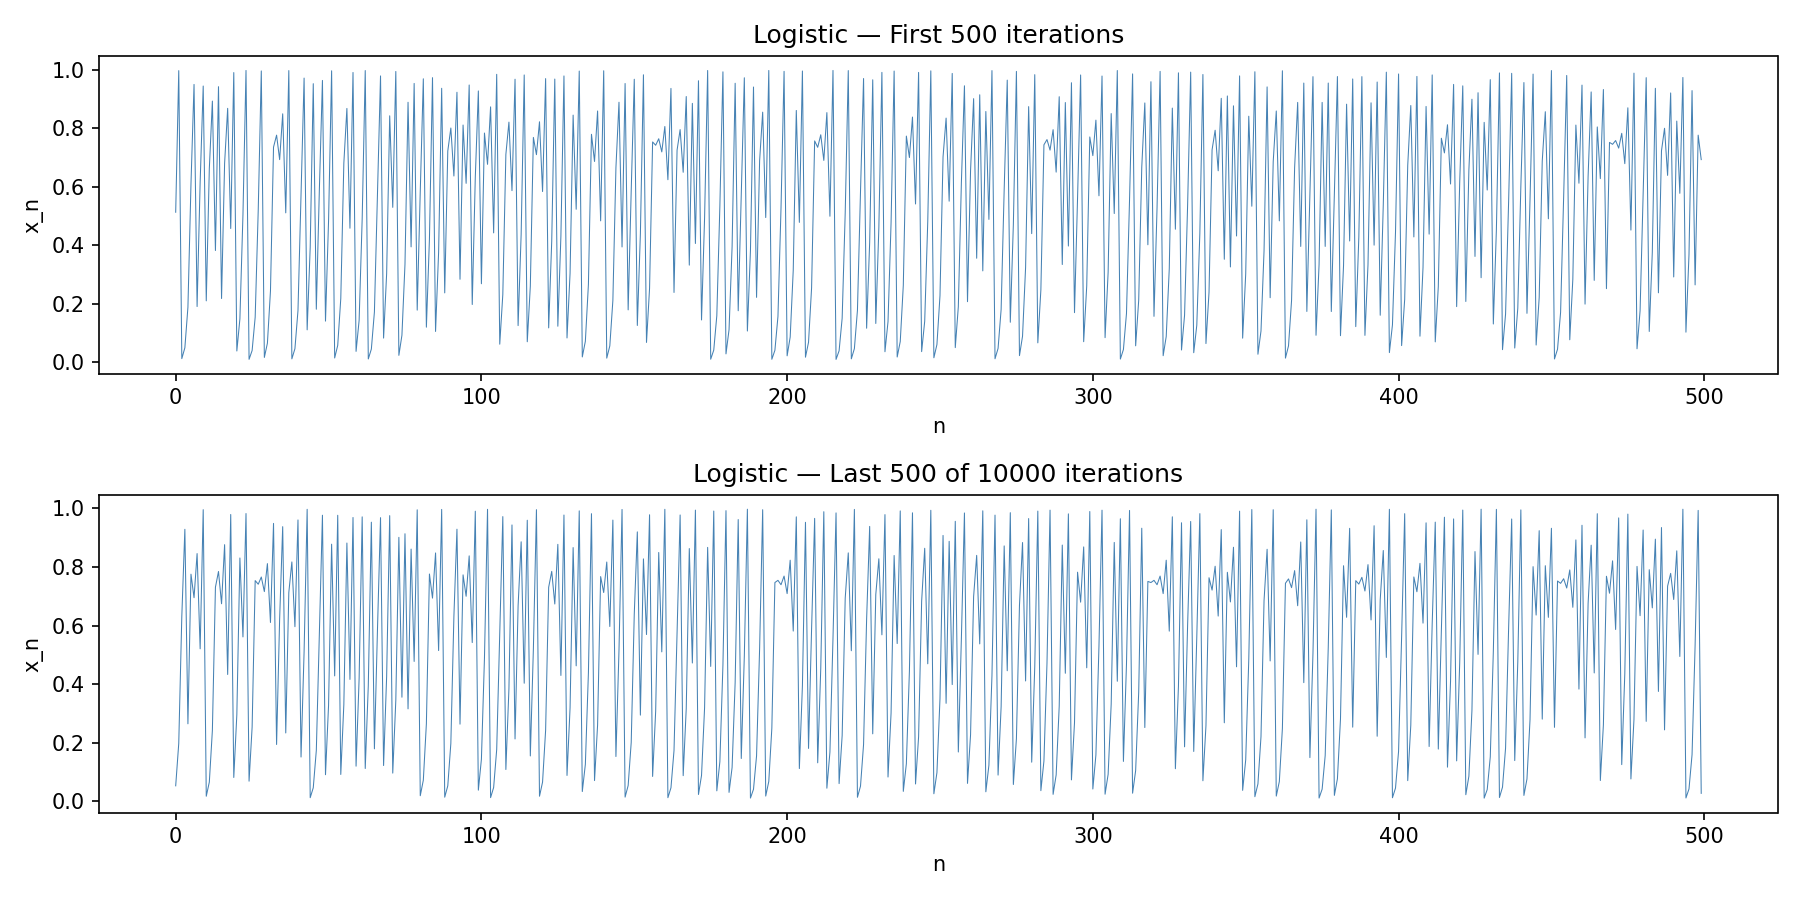
\includegraphics[width=\textwidth]{validation_orbit_logistic.png}
    \caption{Logistic 轨道}
  \end{subfigure}
  \begin{subfigure}[b]{0.48\textwidth}
    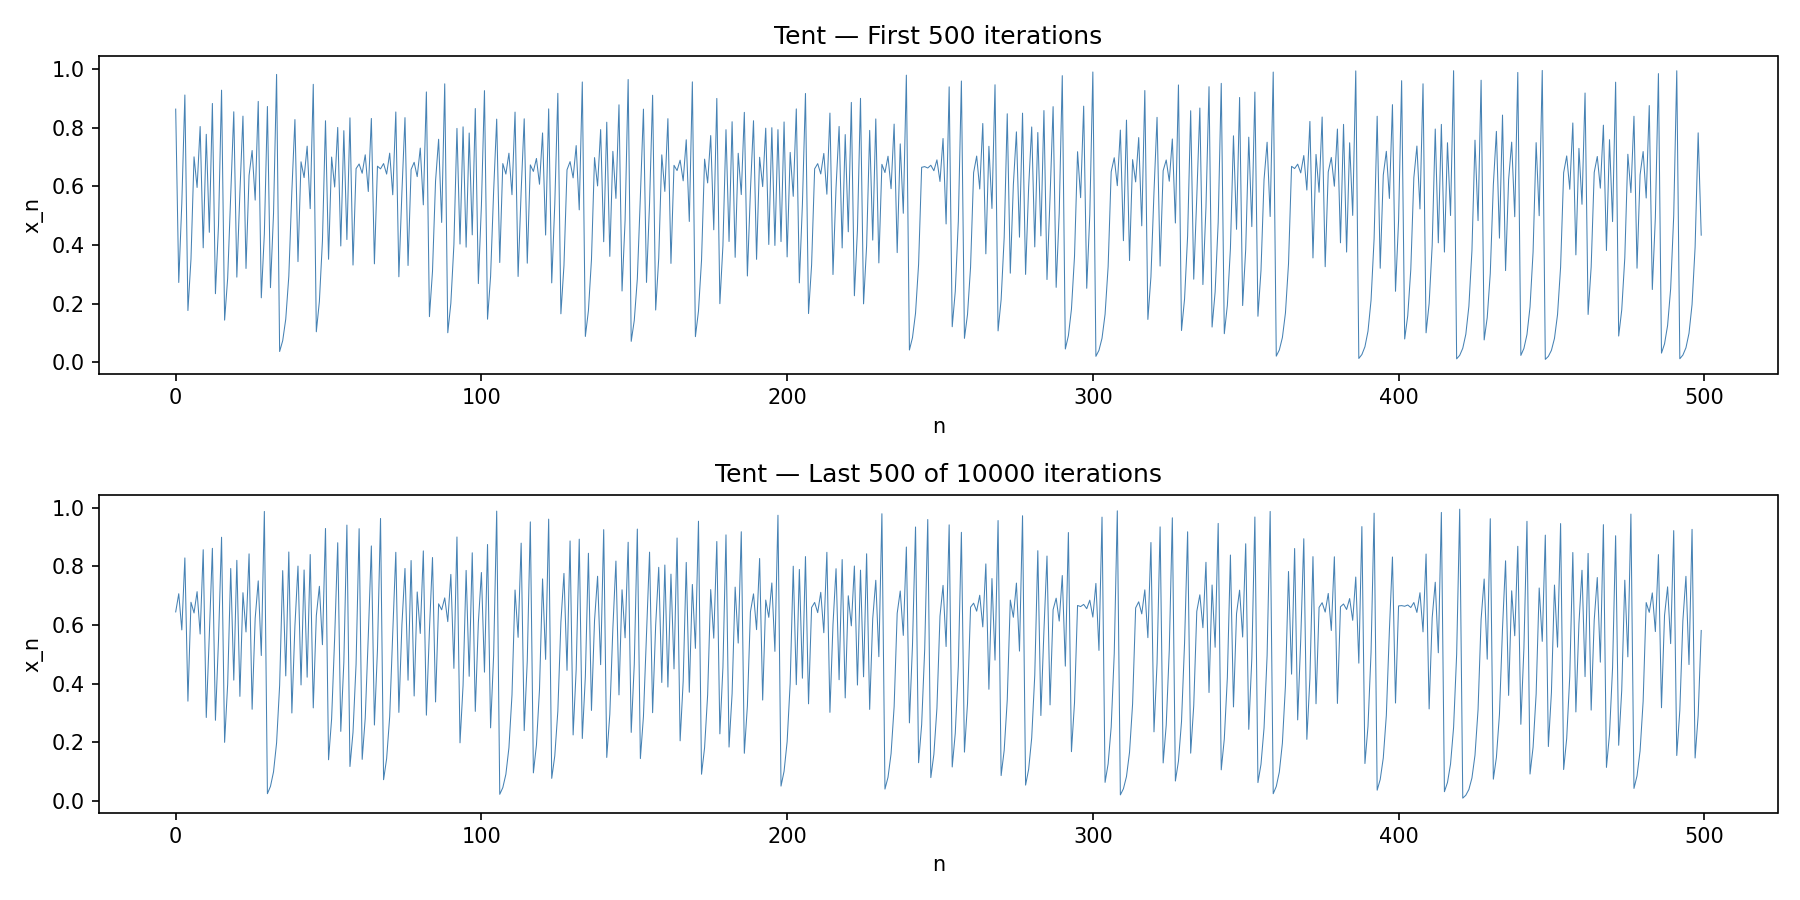
\includegraphics[width=\textwidth]{validation_orbit_tent.png}
    \caption{Tent 轨道}
  \end{subfigure}
  \begin{subfigure}[b]{0.48\textwidth}
    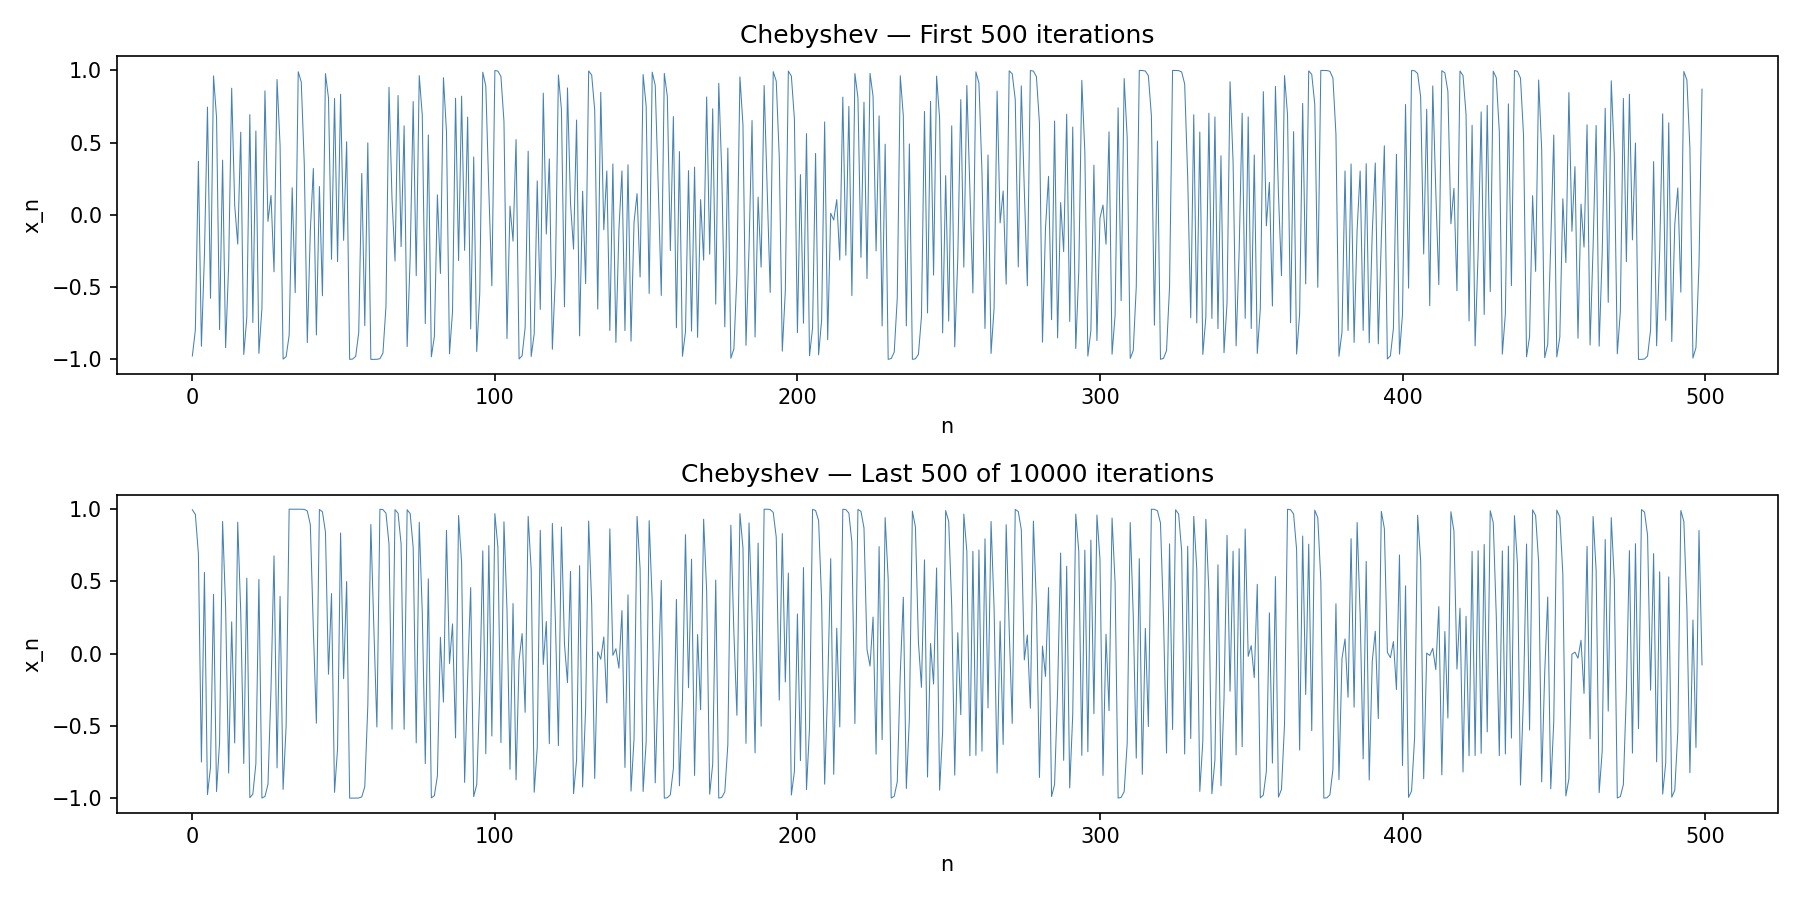
\includegraphics[width=\textwidth]{validation_orbit_chebyshev.png}
    \caption{Chebyshev 轨道}
  \end{subfigure}
  \begin{subfigure}[b]{0.48\textwidth}
    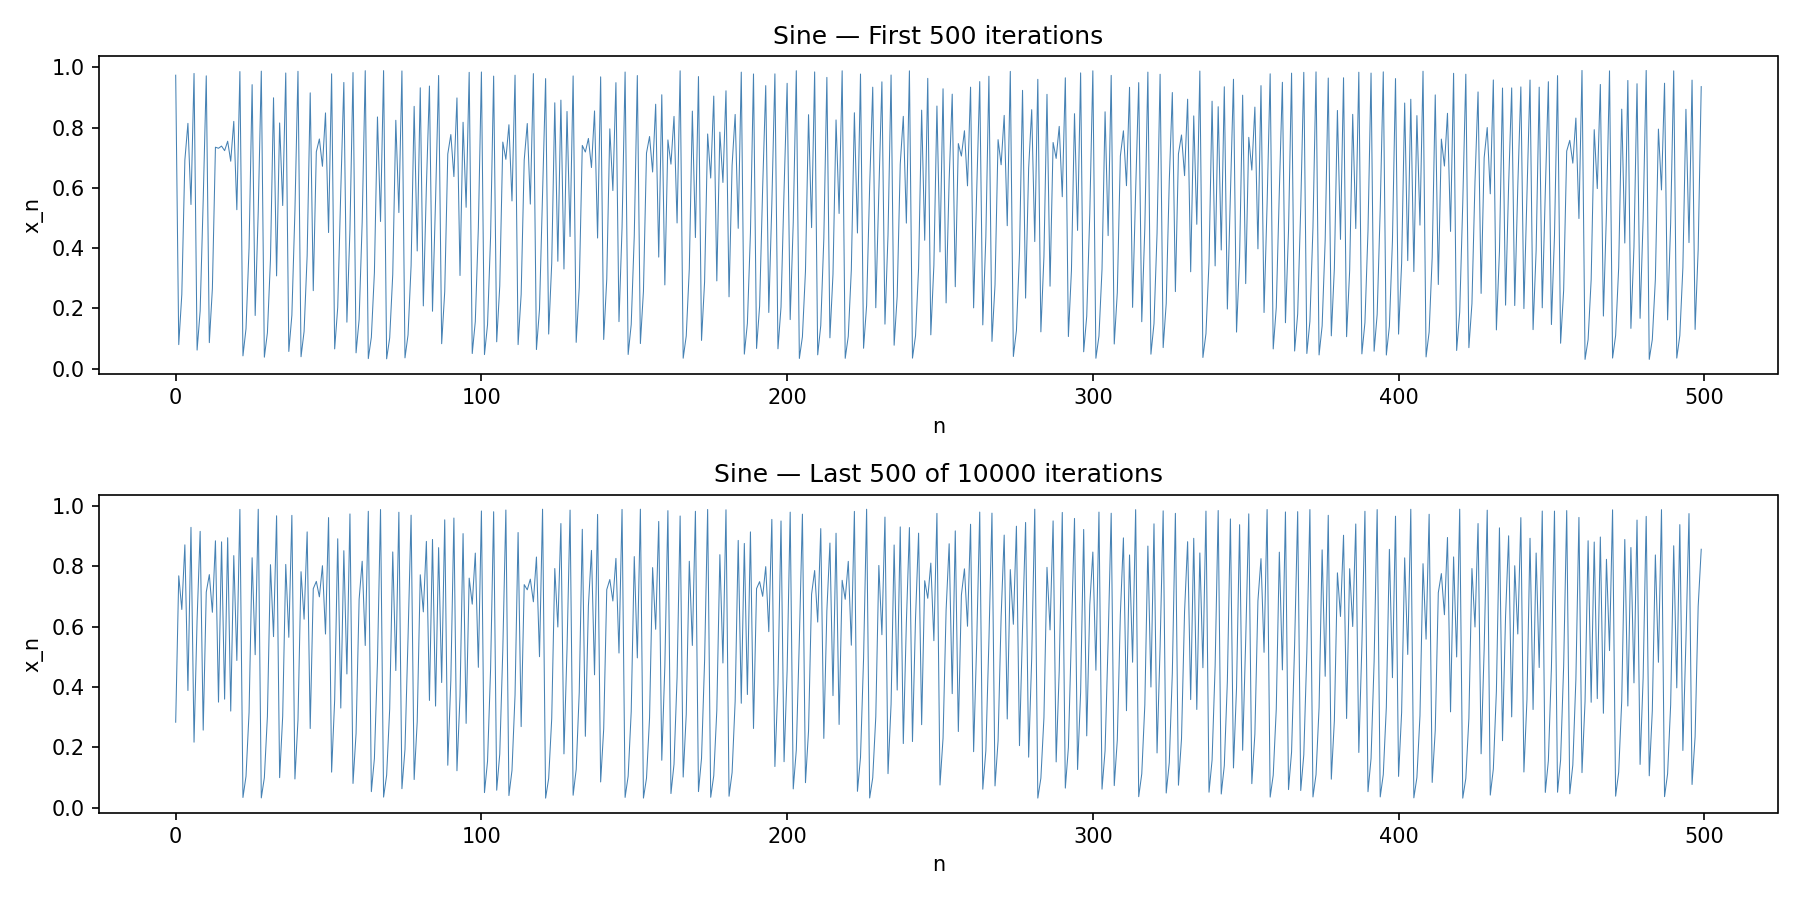
\includegraphics[width=\textwidth]{validation_orbit_sine.png}
    \caption{Sine 轨道}
  \end{subfigure}
  \begin{subfigure}[b]{0.48\textwidth}
    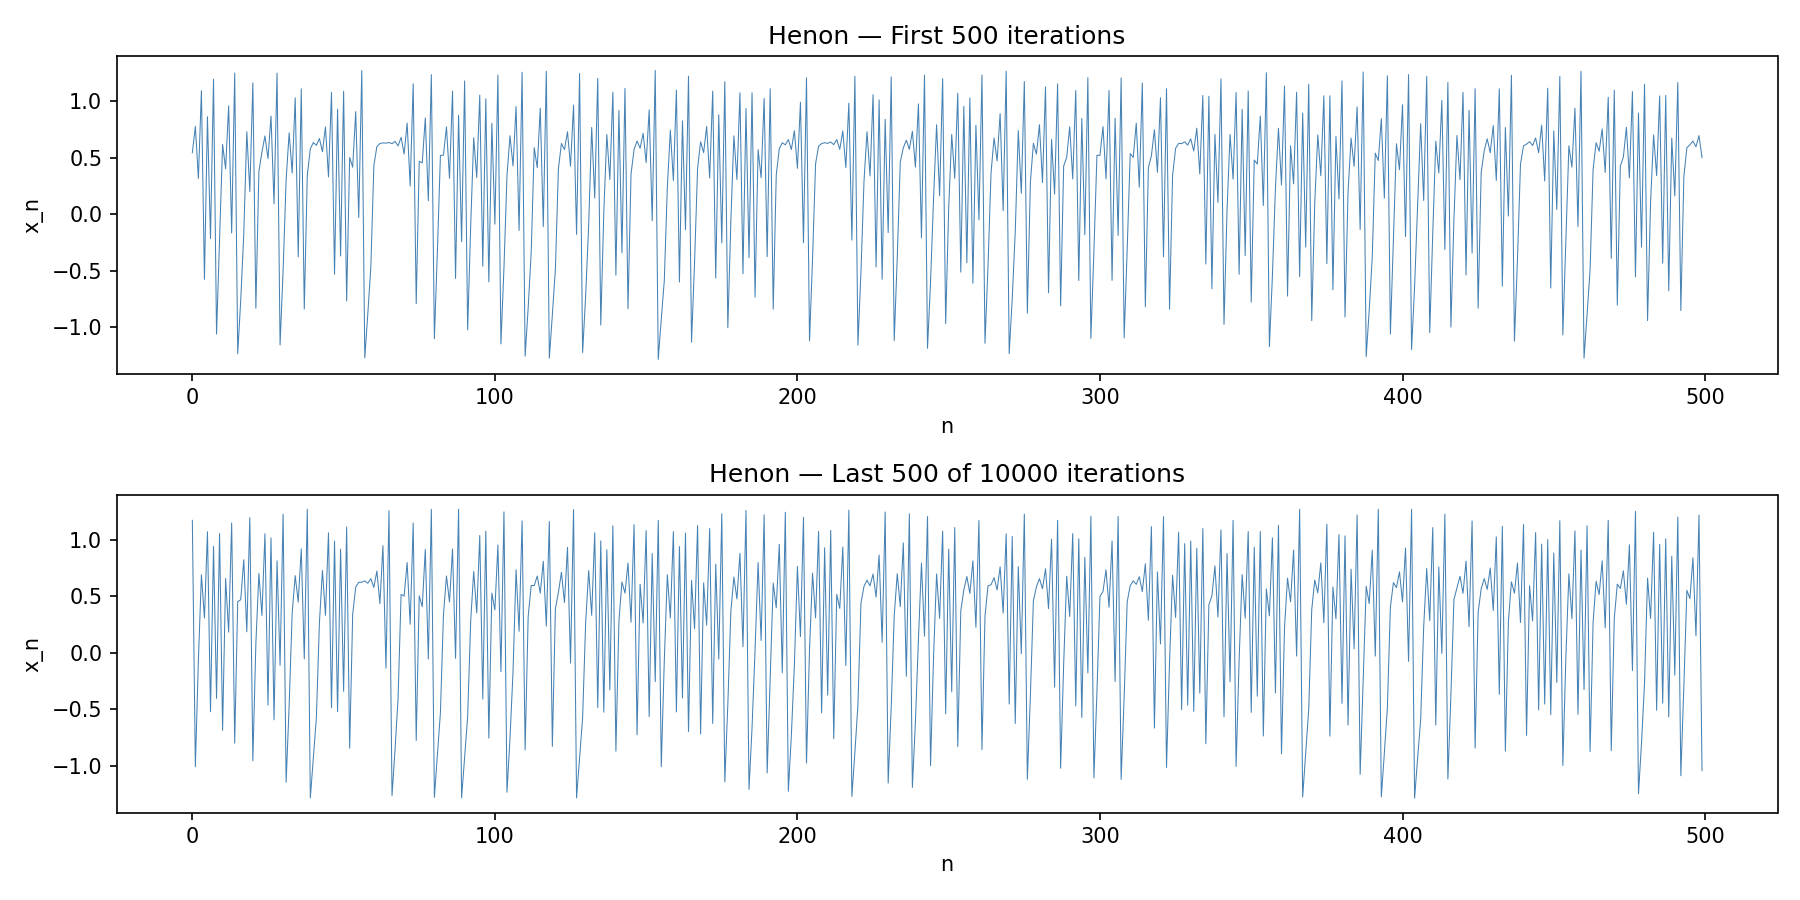
\includegraphics[width=\textwidth]{validation_orbit_henon.png}
    \caption{Henon 轨道}
  \end{subfigure}
  \caption{五种混沌映射的轨道验证图}
  \label{fig:validation}
\end{figure}

\subsection{双射校验}

每张生成的置乱表均通过双射校验：$\text{set}(\pi) = \{0, 1, \ldots, N-1\}$。
经 3500 次以上实验验证，所有映射生成的置乱表均满足双射性，置换表生成正确。

\subsection{Cubic 映射替换说明}

初始设计选用 Cubic 映射（$x_{n+1} = r x_n^2 (1 - x_n)$），
但实验发现该映射在 $r \in [3.8, 3.95]$ 范围内轨道收敛至 0（超稳定不动点），
不满足混沌要求。因此替换为 Sine 映射（$x_{n+1} = r \sin(\pi x_n)$，$r=0.99$），
其混沌行为经验证稳定可靠。

\section{性能测试}

\subsection{参数扫描实验结果}

E4 实验对 Logistic 映射进行参数扫描（$\mu=3.6$ 至 $4.0$，步长 $0.01$，
$N=1024$，每组 30 种子）。结果（图~\ref{fig:param}）显示：

\begin{itemize}
  \item $\mu \in [3.6, 4.0]$ 大部分区间内 $\mathbb{E}[\ln(\text{order})]$ 稳定在 16--20 之间。
  \item 在 $\mu \approx 3.83$ 处出现显著下降：$\mathbb{E}[\ln(\text{order})] = 11.93$，
  标准差仅为 0.60，显著低于相邻参数，对应理论上的周期-3 窗口。
  \item 该发现表明参数选择对循环安全性至关重要，实际应用中应避免 $\mu \approx 3.83$。
\end{itemize}

\begin{figure}[H]
  \centering
  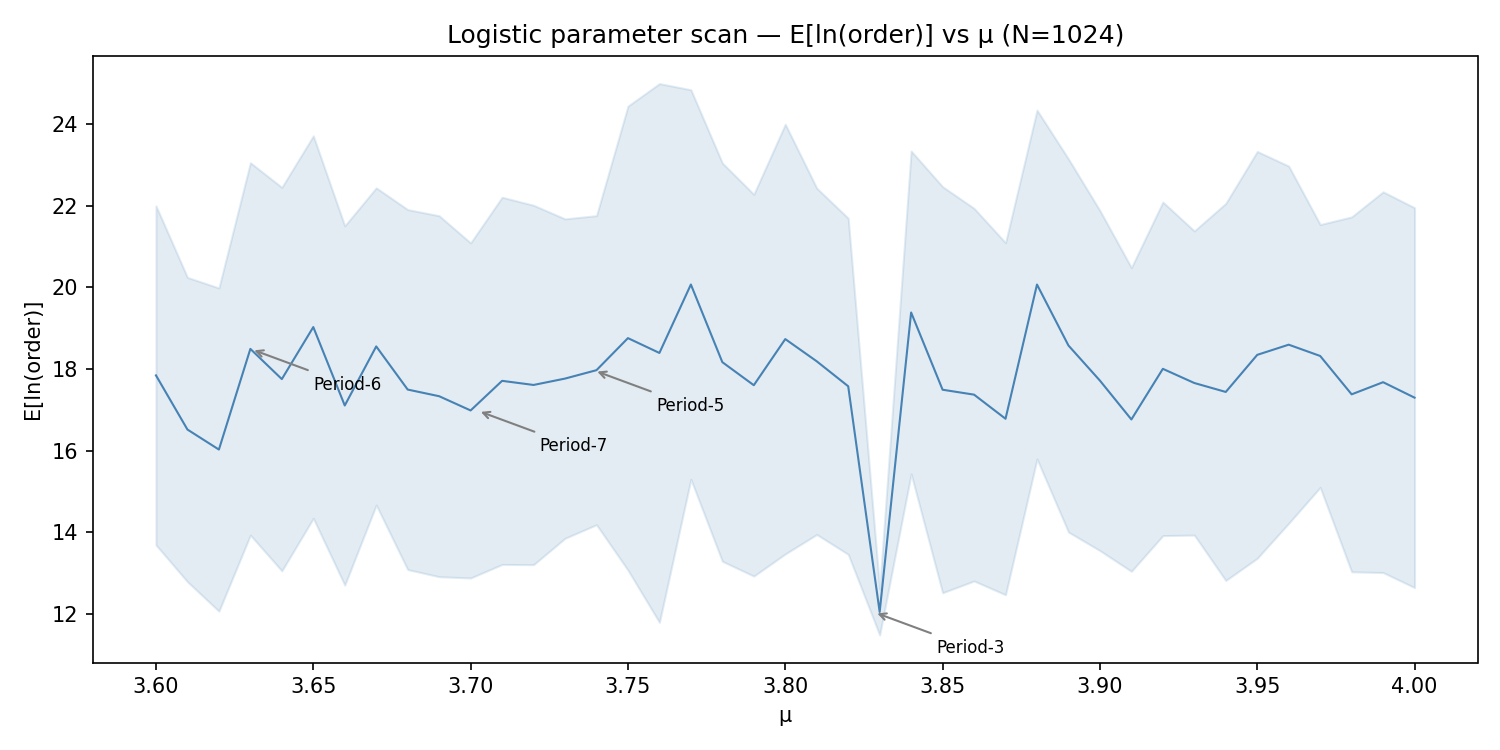
\includegraphics[width=0.85\textwidth]{fig_param_scan_logistic.png}
  \caption{Logistic 映射参数扫描曲线，标注已知周期窗口位置}
  \label{fig:param}
\end{figure}

\section{测试数据与结果}

\subsection{E1/E2：平均阶-N 曲线}

各映射在 $N=1024$ 时的核心统计指标如表~\ref{tab:e1e2} 所示。

\begin{table}[H]
  \centering
  \caption{各映射在 $N=1024$ 时的循环统计指标（100 组种子平均）}
  \label{tab:e1e2}
  \begin{tabular}{lccccc}
    \toprule
    映射 & $\mathbb{E}[\ln O]$ & $\sigma[\ln O]$ & $\mathbb{E}[L_{\max}/N]$ & $\mathbb{E}[C]$ & 固定点比 \\
    \midrule
    Logistic & 18.14 & 4.25 & 0.605 & 7.48 & 0.0010 \\
    Tent & 17.16 & 4.65 & 0.649 & 7.04 & 0.0010 \\
    Chebyshev & 18.10 & 5.00 & 0.646 & 7.46 & 0.0011 \\
    Sine & 17.76 & 4.76 & 0.634 & 7.55 & 0.0008 \\
    Henon & 18.00 & 4.57 & 0.611 & 7.69 & 0.0009 \\
    Fisher-Yates & 18.14 & 4.47 & --- & --- & --- \\
    Landau 参考 & 59.56 & --- & --- & --- & --- \\
    Golomb-Dickman & --- & --- & 0.624 & --- & --- \\
    \bottomrule
  \end{tabular}
\end{table}

分析：
\begin{itemize}
  \item 各映射的 $\mathbb{E}[\ln(\text{order})]$ 与 Fisher-Yates 随机置换（18.14）高度吻合，
  说明混沌置换在阶的统计特性上接近随机置换。
  \item 最大循环比 $\mathbb{E}[L_{\max}/N]$ 在 0.60--0.65 之间，
  与 Golomb-Dickman 常数 0.6243 接近，进一步验证循环结构的随机性。
  \item 固定点比和短循环比均极低（$\ll 0.1\%$），说明没有异常短循环聚集。
\end{itemize}

\subsection{E3：种子初值敏感性}

种子微小扰动（$\epsilon = 10^{-14}$）后的置换差异分析结果见表~\ref{tab:avalanche}。
该实验测量的是混沌置乱对初始条件的敏感程度，与密码学中严格雪崩准则（SAC）含义不同。

\begin{table}[H]
  \centering
  \caption{种子初值敏感性实验结果}
  \label{tab:avalanche}
  \begin{tabular}{lcc}
    \toprule
    映射 & DiffRate & Spearman Footrule \\
    \midrule
    Logistic & 1.000 & 0.687 \\
    Tent & 0.999 & 0.666 \\
    Chebyshev & 1.000 & 0.678 \\
    Sine & 0.996 & 0.673 \\
    Henon & 0.999 & 0.668 \\
    \bottomrule
  \end{tabular}
\end{table}

所有映射的 DiffRate 均接近 1，Footrule 在 0.666--0.687 之间，
说明混沌排序置乱具有极强的初值敏感性。
Logistic 和 Chebyshev 的 DiffRate 达到 1.000（完全置换差异），
表现最为理想。

\subsection{E6：有限精度退化效应}

对比 float32、float64 和 Decimal(50) 三种精度下的置换阶（表~\ref{tab:precision}）。

\begin{table}[H]
  \centering
  \caption{三种精度下 $\mathbb{E}[\ln(\text{order})]$ 对比（$N=256$，30 组种子平均）}
  \label{tab:precision}
  \begin{tabular}{lccc}
    \toprule
    映射 & float32 & float64 & Decimal(50) \\
    \midrule
    Logistic & 10.81 & 10.39 & 11.63 \\
    Tent & 11.92 & 12.05 & 11.47 \\
    Sine & 12.37 & 11.79 & 12.28 \\
    \bottomrule
  \end{tabular}
\end{table}

分析发现：
\begin{itemize}
  \item float32 精度下，部分种子的置换阶退化为 2 或更小，
  说明低精度导致混沌轨道周期化严重，无法产生足够长的置换循环。
  \item float64 和 Decimal(50) 之间的差异较小，
  表明 float64 足以保障循环结构分析的可靠性。
  \item 实际密码应用中，应避免使用 float32 精度的混沌置乱。
\end{itemize}

\subsection{E7：排序法偏差分析}

三组对照（Chaos+argsort、Random+argsort、Fisher-Yates）的对比结果如表~\ref{tab:sorting} 所示。
该实验直接检验：循环结构的特征究竟来自混沌映射本身，还是来自 argsort 操作。

\begin{table}[H]
  \centering
  \caption{排序法偏差分析结果（$N=1024$，60 组种子平均）}
  \label{tab:sorting}
  \begin{tabular}{lccc}
    \toprule
    分组 & $\mathbb{E}[\ln O]$ & $\mathbb{E}[L_{\max}/N]$ & $\mathbb{E}[C]$ \\
    \midrule
    Logistic+argsort & 18.21 & 0.609 & 7.52 \\
    Tent+argsort & 18.22 & 0.586 & 7.22 \\
    Chebyshev+argsort & 18.00 & 0.632 & 7.50 \\
    Sine+argsort & 18.15 & 0.620 & 7.68 \\
    Henon+argsort & 17.32 & 0.678 & 7.43 \\
    Random+argsort & 18.11 & 0.624 & 7.60 \\
    Fisher-Yates & 18.11 & 0.627 & 7.72 \\
    \bottomrule
  \end{tabular}
\end{table}

三组的统计指标极为接近，说明 argsort 操作主导了最终置换的统计特性。
这意味着：在循环结构层面，混沌映射的选择对置换质量的影响有限；
安全性主要依赖于种子空间的密钥规模。

\subsection{E4：参数扫描详细数据}

Logistic 参数扫描的详细数据（部分关键$\mu$值）如表~\ref{tab:param} 所示。

\begin{table}[H]
  \centering
  \caption{Logistic 参数扫描关键数据（$N=1024$，30 组种子平均）}
  \label{tab:param}
  \begin{tabular}{cccc}
    \toprule
    $\mu$ & $\mathbb{E}[\ln O]$ & $\sigma[\ln O]$ & 特征 \\
    \midrule
    3.60 & 17.25 & 4.46 & 混沌区 \\
    3.70 & 17.44 & 4.56 & 混沌区 \\
    3.80 & 17.56 & 4.78 & 混沌区 \\
    \textbf{3.83} & \textbf{11.93} & \textbf{0.60} & \textbf{周期-3 窗口} \\
    3.84 & 20.11 & 3.93 & 恢复正常 \\
    3.90 & 18.10 & 4.79 & 混沌区 \\
    4.00 & 17.50 & 3.64 & 混沌区 \\
    \bottomrule
  \end{tabular}
\end{table}

$\mu=3.83$ 处的阶骤降是 Logistic 映射中周期-3 窗口的典型表现，
说明在该参数下混沌行为失效，置换质量急剧退化。

% ============= 第4章 应用前景 =============
\chapter{应用前景}

基于混沌映射的置乱生成方法在密码学领域具有广阔的应用前景：

\subsection*{图像加密}

混沌排序置乱是图像加密算法中常用的像素位置置乱手段。本作品研究的循环阶分析
可为图像加密方案提供安全性评估依据：若置换阶过小，则加密图像可能在
少量迭代后恢复原图，存在安全隐患。

\subsection*{数据置乱与隐私保护}

在大数据和云计算场景下，数据置乱是保护数据隐私的有效手段。
基于混沌映射的置乱方法具有实现简单、效率高、无需存储完整置换表等优势。
循环阶分析可确保置乱操作具有足够的安全强度。

\subsection*{密码算法设计}

置换操作是许多密码算法的基本构件（如分组密码中的 P-盒）。
混沌映射提供了一种替代性的置换生成方式。本作品的循环分析方法
为评估这类置换的密码学强度提供了系统工具。

\subsection*{工程意义}

本作品的重要发现——float32 精度会严重削弱排序置乱安全性——对工程实现
具有直接指导意义：在实际系统中应至少使用 float64 精度实现混沌置乱。

% ============= 第5章 结论 =============
\chapter{结论}

本作品系统研究了混沌排序置乱的循环阶特性，主要发现如下：

\subsection*{主要发现}

\begin{enumerate}
  \item \textbf{循环结构接近均匀随机置换}：五种混沌排序置乱在
  $\mathbb{E}[\ln(\text{order})]$、最大循环比、循环数等指标上
  与 Fisher-Yates 基线高度接近。Landau 上界参考线（$S_N$ 中最大可能阶）
  与实验值存在较大差距，说明实际阶远未达到理论上限。
  
  \item \textbf{具备强初值敏感性}：种子微扰下置换差异率接近 1，
  Spearman Footrule 在 0.66--0.69 之间。
  但需注意：初值敏感性不等同于密码学严格雪崩准则（SAC）。
  
  \item \textbf{argsort 主导统计特性}：Chaos+argsort 与 Random+argsort、
  Fisher-Yates 三组对照结果高度一致，说明 argsort 操作主导了最终
  置换的统计特性，混沌映射选择在循环结构层面的影响有限。
  
  \item \textbf{低精度导致安全退化}：float32 精度下混沌轨道提前周期化，
  置换阶显著降低，应避免在密码应用中使用。
  
  \item \textbf{参数选择关键}：Logistic 映射在 $\mu \approx 3.83$ 处
  存在周期窗口，参数选择不当将导致安全性急剧下降。
\end{enumerate}

\subsection*{安全性评价}

综合 Q1--Q9 安全指标，五种混沌映射的安全性排序为：
$$
  \text{Logistic} \approx \text{Chebyshev} \approx \text{Henon}
  \approx \text{Sine} \approx \text{Tent}
$$
在循环结构层面，各映射之间不存在本质差异。
混沌排序置乱的安全性主要来源于种子密钥空间的规模，
而非特定映射类型的循环结构特征。低阶意味着重复置乱后更快回归恒等映射，
有效置乱空间随阶降低而缩减——这是循环阶分析的核心安全含义。

\subsection*{局限性}

\begin{itemize}
  \item 本作品仅分析了置换的循环结构，未涉及其他安全性指标
  （如相关免疫性、代数次数等）。
  \item 参数扫描仅针对 Logistic 映射，未覆盖其他映射的参数空间。
  \item Decimal(50) 精度实验限于 Logistic、Tent、Sine 三种多项式型映射。
\end{itemize}



\end{document}
